\documentclass[10pt]{beamer}
\usepackage[utf8]{inputenc}
\usepackage[T1]{fontenc}
\usepackage{graphicx}
\usepackage{amsmath}
\usepackage{hyperref}

\title{Viva Melhor}
\author{Omeir Haroon 61810}
\date{\today}

\begin{document}

\begin{frame}
    \titlepage
\end{frame}

\section{Introdução}
\begin{frame}{Introdução}
    \begin{itemize}
        \item Seguro de saúde refere-se a um tipo de "proteção" que pessoas podem obter para ajudar a pagar por serviços médicos.
        \item É importante porque quem tem preocupa-se menos com os custos de assistência médica.
    \end{itemize}

    \begin{quote}
        "No one plans to get sick or hurt, but most people need medical care at some point. Health insurance covers these costs and offers many other important benefits." \cite{healthcare}
    \end{quote}
\end{frame}

\begin{frame}{Vantagens e Desvantagens de seguro de saúde}
    \begin{columns}
        \column{0.5\textwidth}
        \begin{block}{Vantagens}
            \begin{itemize}
                \item Independência
                \item Liberdade de escolha
                \item Tempo de espera
            \end{itemize}
        \end{block}

        \column{0.5\textwidth}
        \begin{block}{Desvantagens}
            \begin{itemize}
                \item Custo
                \item Exclusões
                \item Franquia
            \end{itemize}
        \end{block}
    \end{columns}
\end{frame}

\section{Caso de Estudo}
\begin{frame}{Caso de Estudo}
    \begin{quote}
        A Declaração Universal dos Direitos Humanos garante saúde e um nível de vida adequado. Em Portugal, o SNS é universal e frequentemente gratuito. Devido à demanda, a iniciativa privada oferece seguros de saúde. Nelson avalia três propostas de uma Companhia de Seguros, a serem registradas na tabela (exemplo: 61810).
    \end{quote}
\end{frame}

\begin{frame}{Tabela de preços dos três tipos de seguros}
    \begin{table}
        \centering
        \begin{tabular}{|c|c|}
            \hline
            \textbf{Vantagens} & \textbf{Desvantagens} \\
            \hline
            Independência & Custo \\
            \hline
            Liberdade de escolha & Exclusões \\
            \hline
            Tempo de espera & Franquia \\
            \hline
        \end{tabular}
        \caption{Vantagens e Desvantagens de seguro de saúde}
    \end{table}
\end{frame}

\begin{frame}{Comparação dos preços em relação ao número de atos médicos}
    \begin{table}
        \centering
        \begin{tabular}{|l|l|l|l|}
            \hline
            Nº Atos Médicos Anuais & Seguro A & Seguro B & Seguro C \\
            \hline
            10 & 0 & 0 & 0 \\
            20 & 82 & 21 & 0 \\
            30 & 164 & 63 & 100 \\
            40 & 246 & 105 & 200 \\
            50 & 328 & 147 & 300 \\
            60 & 410 & 189 & 400 \\
            70 & 492 & 231 & 500 \\
            80 & 574 & 273 & 600 \\
            90 & 656 & 315 & 700 \\
            \hline
        \end{tabular}
        \caption{Comparação dos preços em relação ao número de atos médicos}
    \end{table}
\end{frame}

\begin{frame}{Comparação de seguros de saúde}
    \begin{figure}
        \centering
        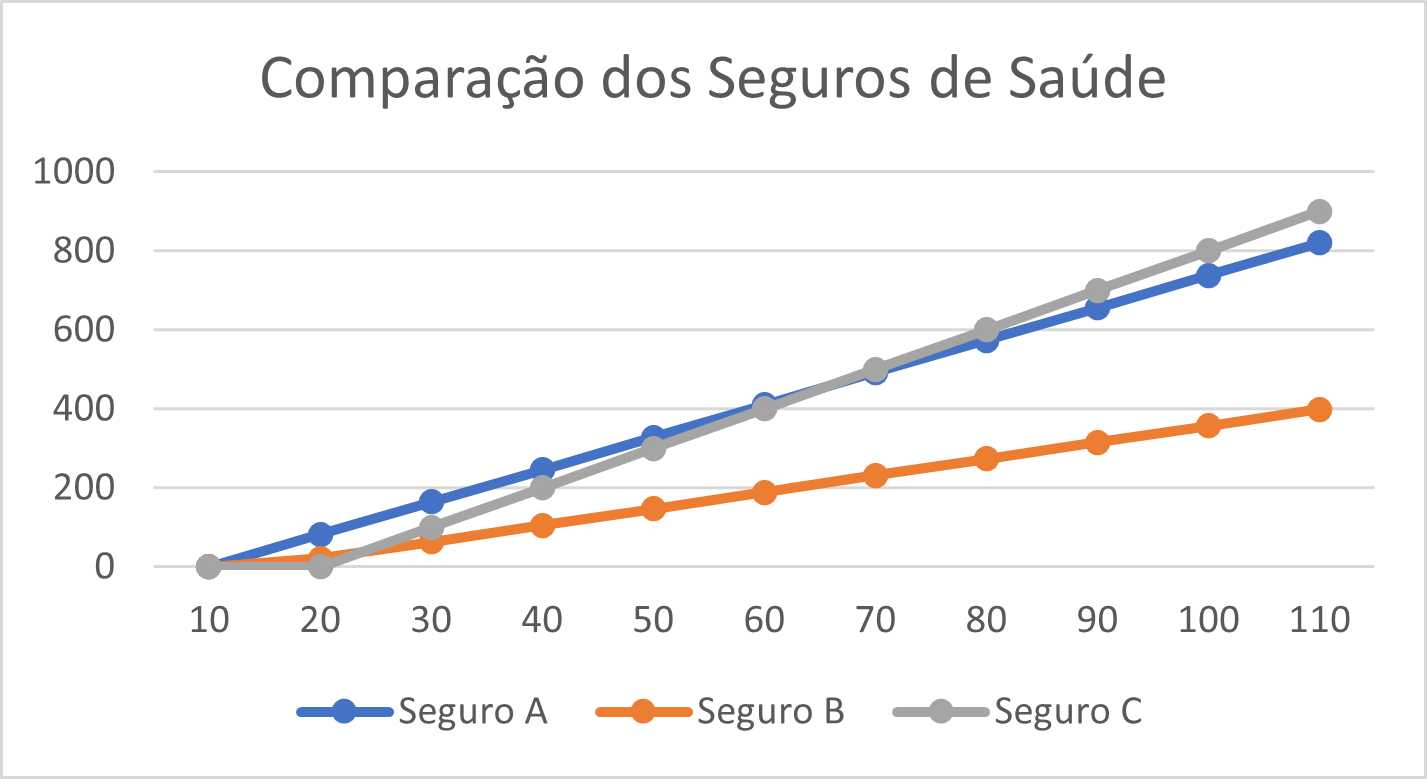
\includegraphics[scale=0.5]{graph}
        \caption{Comparação de seguros de saúde}
    \end{figure}
\end{frame}

\section{Conclusão}
\begin{frame}{Conclusão}
    \begin{itemize}
        \item Custo vs. Benefício: O Seguro B apresenta a menor anuidade e tarifas de atos médicos, tornando-o uma opção mais acessível.
        \item Cobertura de Atos Médicos: O Seguro C oferece uma ampla cobertura de atos médicos, especialmente para valores mais altos.
        \item Liberdade de Escolha: Todos os seguros oferecem liberdade de escolha, mas o Seguro C pode ser mais atrativo devido à sua cobertura abrangente.
        \item Ponderação Pessoal: A escolha entre os seguros deve ser baseada nas necessidades específicas do senhor Nelson e sua família.
    \end{itemize}
\end{frame}

\begin{frame}{Bibliografia}
    \begin{thebibliography}{9}
        \bibitem{healthcare}
        HealthCare.gov. "Why Coverage is Important." [Online]
        Available: \url{https://www.healthcare.gov/why-coverage-is-important}
    \end{thebibliography}
\end{frame}

\end{document}
